\documentclass{article}
\usepackage{graphicx}
\usepackage[margin=1.5cm]{geometry}
\usepackage{amsmath}

\begin{document}

\title{Thursday Reading Assessment: Unit 4, AC waveforms}
\author{Prof. Jordan C. Hanson}

\maketitle

\section{Memory Bank}

\begin{itemize}
\item $v(t) = v_0 \sin(2\pi ft - \phi)$ ... Standard AC waveform, with amplitude $v_0$, in volts, frequency $f$, in Hertz, time $t$, in seconds, and phase $\phi$, in radians.
\item Note that the relative phase between the sine function and the cosine function is 90 degrees.
\end{itemize}

\section{Properties of AC Waveforms}

\begin{figure}
\centering
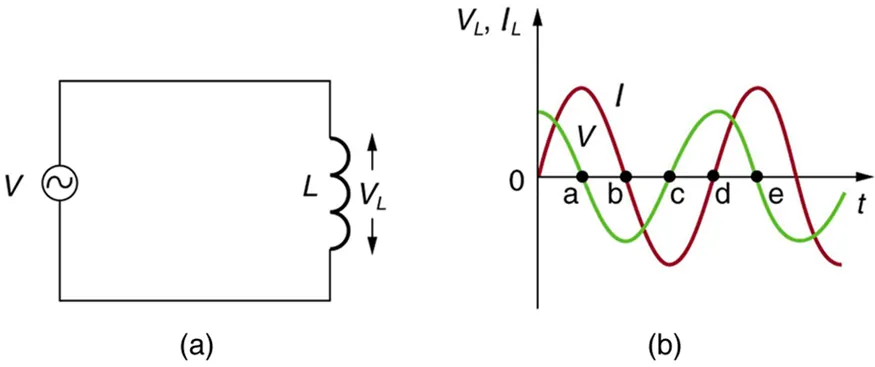
\includegraphics[width=0.65\textwidth]{figures/phase.png}
\caption{\label{fig:1} AC waveforms of voltage and current versus time.}
\end{figure}

\begin{enumerate}
\item Consider the voltage waveform in Fig. \ref{fig:1}.  The voltages at points a, c, and e, are zero.  Suppose that $t_a = 1$ ms, and $t_e = 3$ ms. (a) What is the period of the voltage? (b) What is the frequency of the voltage? \\ \vspace{2cm}
\item While the amplitude of the voltage at time $t_a$ is zero, the amplitude of the current is maximized.  (a) What is the relative phase between the two waveforms? (c) If two waveforms have a relative phase shift of 180 degrees, what happens when they are summed? \textit{Hint: try creating an example.}\\ \vspace{2cm}
\item (a) If a signal has a frequency of 10 kHz, what is its period? (b) If the period of a signal is 2 $\mu$s, what is the frequency? (c) If the period of 2 $\mu$s is \textit{doubled}, what is the frequency?
\end{enumerate}
\end{document}
